% !TeX root = ../main.tex
% Add the above to each chapter to make compiling the PDF easier in some editors.

\chapter{Background}\label{chapter:background}

The understanding of the LAIK library and Inter Process Communication (IPC) is fundamental for understanding the design of the shared memory Backend. This chapter is divided into two parts. In the first, we will briefly introduce the basic features of LAIK, with particular emphasis on action sequences, backend interface, and data storage. In the second part we will cover the necessary basics of inter process communication, especially shared memory and semaphores.

\section{LAIK}

LAIK, which stands for \glqq Leichtgewichtige AnwendungsIntegriete Datenhaltungskomponente\grqq, is a library for data management in the HPC environment. Created out of the need for higher flexibility in regard to scheduling and fault tolerance strategies, LAIK provides support for distributing data across parallel applications by controlling the data and its partitioning. The goal of LAIK is to provide fault tolerance mechanisms and load balancing for HPC applications in the most lightweight and performant way possible \cite{laik-paper}. As shown in fig.\ref{fig:laik-layers}, LAIK sits between the actual application and the library used for communication.

\begin{figure}[h]
	\centering
	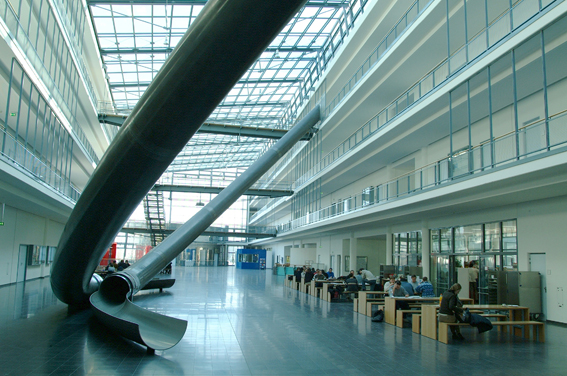
\includegraphics[scale=0.5]{figures/tum.jpg}
	\caption{LAIK and Communication Backend}
	\label{fig:laik-layers}
\end{figure}

\subsection{Action Sequences}

Action sequences are a list of actions which provide the information a node needs to execute a specific chain of actions. Actions are the atomic unit of execution in LAIK, they are predefined procedures which contain the necessary information for their own execution. LAIK creates action sequences based on the applications needs. After a sequence is created it can be optimised before it is executed. When an Action sequence is executed, the corresponding backend performs every Action of the sequence in the determined order. Action sequences can be executed multiple times. When an action sequence isn't needed anymore, it gets deleted.

\subsection{Backend Interface}

As per its specification, LAIK supports different communication libraries to execute the data migration \cite{laik-paper}. Application programmers are able to

% What is a backend

% What methods does the interface have


\subsection{Data Storage}

% How is data stored in LAIK

% What is an Allocator


\section{Inter Process Communication}

% What is IPC

% Which type is necessary for our project

\subsection{Shared memory}

% What is shared memory

% How does SysV shared memory work

\subsection{Semaphores}

% What is a semaphore

% How do SysV semaphores work